\documentclass[12pt]{thesis-NJFU}

\title{关于thesis-NJFU项目的快速上手、}
{基本介绍、示例以及测试文档}{A Quick Start and Introduction to thesis-NJFU, 
with Corresponding Demonstrations and Tests}
\college{理学院}
\major{信息与计算科学}
\class{1811011}
\studentnumber{181101181}
\author{ty}
\advisor{你的指导老师}
\advisortitle{副教授}

\begin{document}

\makecover

\copyrightpage

\begin{cnabstract}
{\normalsize 字}{\fontsize{12pt}{0pt}\selectfont 字12pt}
{\normalsize 字}{\fontsize{10pt}{0pt}\selectfont 字10pt}
{\normalsize 字}{\fontsize{10.5pt}{0pt}\selectfont 字10.5pt}
{\normalsize 字}{\fontsize{11pt}{0pt}\selectfont 字11pt}

摘要摘要摘要摘要摘要摘要摘要摘要摘要摘要摘要摘要摘要摘要摘要摘要摘要摘要摘要摘要摘要摘要摘要摘要摘要摘要摘要摘要
摘要摘要摘要摘要摘要摘要摘要摘要摘要摘要摘要摘要摘要摘要摘要摘要摘要摘要摘要摘要摘要摘要摘要摘要摘要摘要摘要摘要摘要摘要摘要摘要摘要摘要摘要摘要摘要摘要摘要摘要摘要摘要
摘要摘要摘要摘要摘要摘要摘要摘要摘要摘要摘要摘要摘要摘要摘要摘要摘要摘要摘要摘要摘要摘要摘要摘要摘要摘要摘要摘要

摘要摘要摘要摘要摘要摘要摘要摘要摘要摘要摘要摘要摘要摘要摘要摘要摘要摘要摘要摘要摘要摘要摘要摘要摘要摘要摘要摘要
摘要摘要摘要摘要摘要摘要摘要摘要摘要摘要摘要摘要摘要摘要摘要摘要摘要摘要摘要摘要摘要摘要摘要摘要摘要摘要摘要摘要
摘要摘要摘要摘要摘要摘要摘要摘要摘要摘要摘要摘要摘要摘要摘要摘要摘要摘要摘要摘要摘要摘要摘要摘要摘要摘要摘要摘要
摘要摘要摘要摘要摘要摘要摘要摘要摘要摘要摘要摘要摘要摘要摘要摘要摘要摘要摘要摘要摘要摘要摘要摘要摘要摘要摘要摘要
摘要摘要摘要摘要摘要摘要摘要摘要摘要摘要摘要摘要摘要摘要摘要摘要摘要摘要摘要摘要摘要摘要摘要摘要摘要摘要摘要摘要
摘要摘要摘要摘要摘要摘要摘要摘要摘要摘要摘要摘要摘要摘要摘要摘要摘要摘要摘要摘要摘要摘要摘要摘要摘要摘要摘要摘要

摘要摘要摘要摘要摘要摘要摘要摘要摘要摘要摘要摘要摘要摘要摘要摘要摘要摘要摘要摘要摘要摘要摘要摘要摘要摘要摘要摘要

注意:在开始关键词环境时与摘要内容不要空行!
\begin{cnkeywords}
关键词1;关键词2;关键词3;关键词4
\end{cnkeywords}
\end{cnabstract}

\begin{enabstract}
	abstract abstract abstract abstract abstract abstract abstract abstract abstract abstract abstract abstract abstract abstract abstract abstract abstract abstract abstract abstract 
	abstract abstract abstract abstract abstract abstract abstract abstract abstract abstract abstract abstract abstract abstract abstract abstract abstract abstract abstract abstract 
	abstract abstract abstract abstract abstract abstract abstract abstract abstract abstract abstract abstract abstract abstract abstract abstract abstract abstract abstract abstract 
	abstract abstract abstract abstract abstract abstract abstract abstract abstract abstract abstract abstract abstract abstract abstract abstract abstract abstract abstract abstract 
	abstract abstract abstract abstract abstract abstract abstract abstract abstract abstract abstract abstract abstract abstract abstract abstract abstract abstract abstract abstract 

	abstract abstract abstract abstract abstract abstract abstract abstract abstract abstract abstract abstract abstract abstract abstract abstract abstract abstract abstract abstract 
	abstract abstract abstract abstract abstract abstract abstract abstract abstract abstract abstract abstract abstract abstract abstract abstract abstract abstract abstract abstract 
	abstract abstract abstract abstract abstract abstract abstract abstract abstract abstract abstract abstract abstract abstract abstract abstract abstract abstract abstract abstract 
	abstract abstract abstract abstract abstract abstract abstract abstract abstract abstract abstract abstract abstract abstract abstract abstract abstract abstract abstract abstract 

	abstract abstract abstract abstract abstract abstract abstract abstract abstract abstract abstract abstract abstract abstract abstract abstract abstract abstract abstract abstract 
	abstract abstract abstract abstract abstract abstract abstract abstract abstract abstract abstract abstract abstract abstract abstract abstract abstract abstract abstract abstract 
\begin{enkeywords}
	Ant Colony Algorithm;Dynamic programming model;TSP problem;Coupled storage mode
\end{enkeywords}
\end{enabstract}

\tableofcontents

\mainpart

\section{从这里开始}
正文开始前请使用\verb|\mainpart|命令.
\subsection{注意:Before you start}
在开始前,请确认你正在使用现代化的能够正常自动补全宏包的编译器,包括但不局限于:MikTeX, TexLive.
请注意:使用outdated的MikTeX作为编译器的CTeX套件恕不受支持(虽然很多人以该套件入门).
本项目当前版本为\verb|v1.0|,仅在Windows上的编译器测试通过,使用UTF-8编码.

编译时请使用XeLaTeX,参考文献使用Biber引擎.

确保你已经安装华文中宋与仿宋字体.

另外, 本文档面向具有\LaTeX 基础的写作人群, 基础的\LaTeX 语法请参阅相关教程文档.

\subsection{快速上手}

使用\verb|\documentclass[12pt]{thesis-NJFU}|命令来使用本项目.

\subsubsection{基本信息}
在插入封面前,请使用相关命令定义基本信息.本文的定义如下:
\begin{verbatim}
\title{关于thesis-NJFU项目的快速上手、}
{基本介绍、示例以及测试文档}
{A Quick Start and Introduction to thesis-NJFU, 
with Corresponding Demonstrations and Tests}
\college{理学院}
\major{信息与计算科学}
\class{1811011}
\studentnumber{181101181}
\author{ty}
\advisor{你的指导老师}
\advisortitle{副教授}
\end{verbatim}
其中,\verb|\title|命令接收3个参数:中文标题头,中文标题尾和英文标题.中文标题头和中文标题尾构成完整的中文标题.
使用\verb|\college|定义学院,\verb|\major|命令定义专业,
\verb|\class|命令定义班级,\verb|\studentnumber|命令定义学号,\verb|\author|命令定义作者姓名,
\verb|\advisor|命令定义指导老师姓名,\verb|\advisortitle|命令定义指导老师职称.

\subsubsection{写作流程}
在定义完基本信息后,使用\verb|\makecover|命令绘制封面.
注意中文标题头和中文标题尾会被分别填入封面标题的第1,第2行.
封面将自动填写中文格式日期.

thesis-NJFU使用\verb|cnabstract|和\verb|enabstract|环境分别提供中、英文摘要.
在中、英文摘要中,分别提供\verb|cnkeywords|和\verb|enkeywords|环境来显示关键词.
注意,使用两种关键词环境时不要与摘要内容之间存在空行,即不要另起一段!
thesis-NJFU会自动在摘要中创建标题以及"摘要"、"ABSTRACT"字样.

在摘要结束后,使用\verb|\tableofcontents|命令绘制目录.注意目录在更改时需要两次编译才可以正常显示.

在开始正文前,请使用\verb|\mainpart|命令调整文章样式至正文部分.

对于结论和致谢二部分,thesis-NJFU分别提供\verb|\conclusion|和\verb|\acknowledgement|命令创建内容.
这些部分不会被编号,但会被收录在目录中.

最后,使用\verb|\thesisreferences|命令来打印参考文献.文献管理请使用biber语法, 可参阅\verb|references.bib|文件内容.
推荐使用Google Scholar导出bibtex格式引用.thesis-NJFU将自动按照GB/T 7714-2015 标准按照引用顺序编写参考文献条目.

\verb|\copyrightpage|命令用来创建本项目的版权页, 可根据需求删去或保留:)

\subsection{项目所使用的部分宏包}

\subsubsection{中文环境实现}

基础宏包不再赘述.中文环境以article类为基础配合\verb|ctex|实现.

中文日期采用\verb|datetime|宏包和\verb|zhumber|宏包实现.

\subsubsection{参考文献实现}

NJFU要求以GB/T 7714-2015 标准编写参考文献条目.
thesis-NJFU使用\verb|biblatex|宏包的Biber引擎,并使用胡振震(Email:\url{ hzzmail@163.com})
编写的"符合 GB/T 7714-2015 标准的 biblatex 参考文献样式包"(available at \url{https://github.com/hushidong/biblatex-gb7714-2015})实现.

\subsubsection{标题样式实现}

对于图表标题样式,thesis-NJFU使用\verb|caption|宏包实现;对于章节标题样式,thesis-NJFU使用\verb|titlesec|宏包实现;对于目录样式,使用\verb|titletoc|宏包实现.

\subsection{关于查重}

经测试thesis-NJFU在包括知网等查重系统中表现正常, 无乱码现象.

\section{示例}

\subsection{引用示例}
示例一\cite{ShiShengjun}:\verb|\cite{ShiShengjun}|

示例二\authornumcite{PMID:24476821}:\verb|\authornumcite{PMID:24476821}|

示例三\cite{GEO,ShiShengjun}:\verb|\cite{GEO,ShiShengjun}|

相关文献的entry请在\verb|references.bib|中录入\footnote{To get citations right, run XeLaTeX -> biber -> XeLaTeX -> XeLaTeX in order.}.

\subsection{图片示例}
\begin{figure}[htbp]
	\centering
	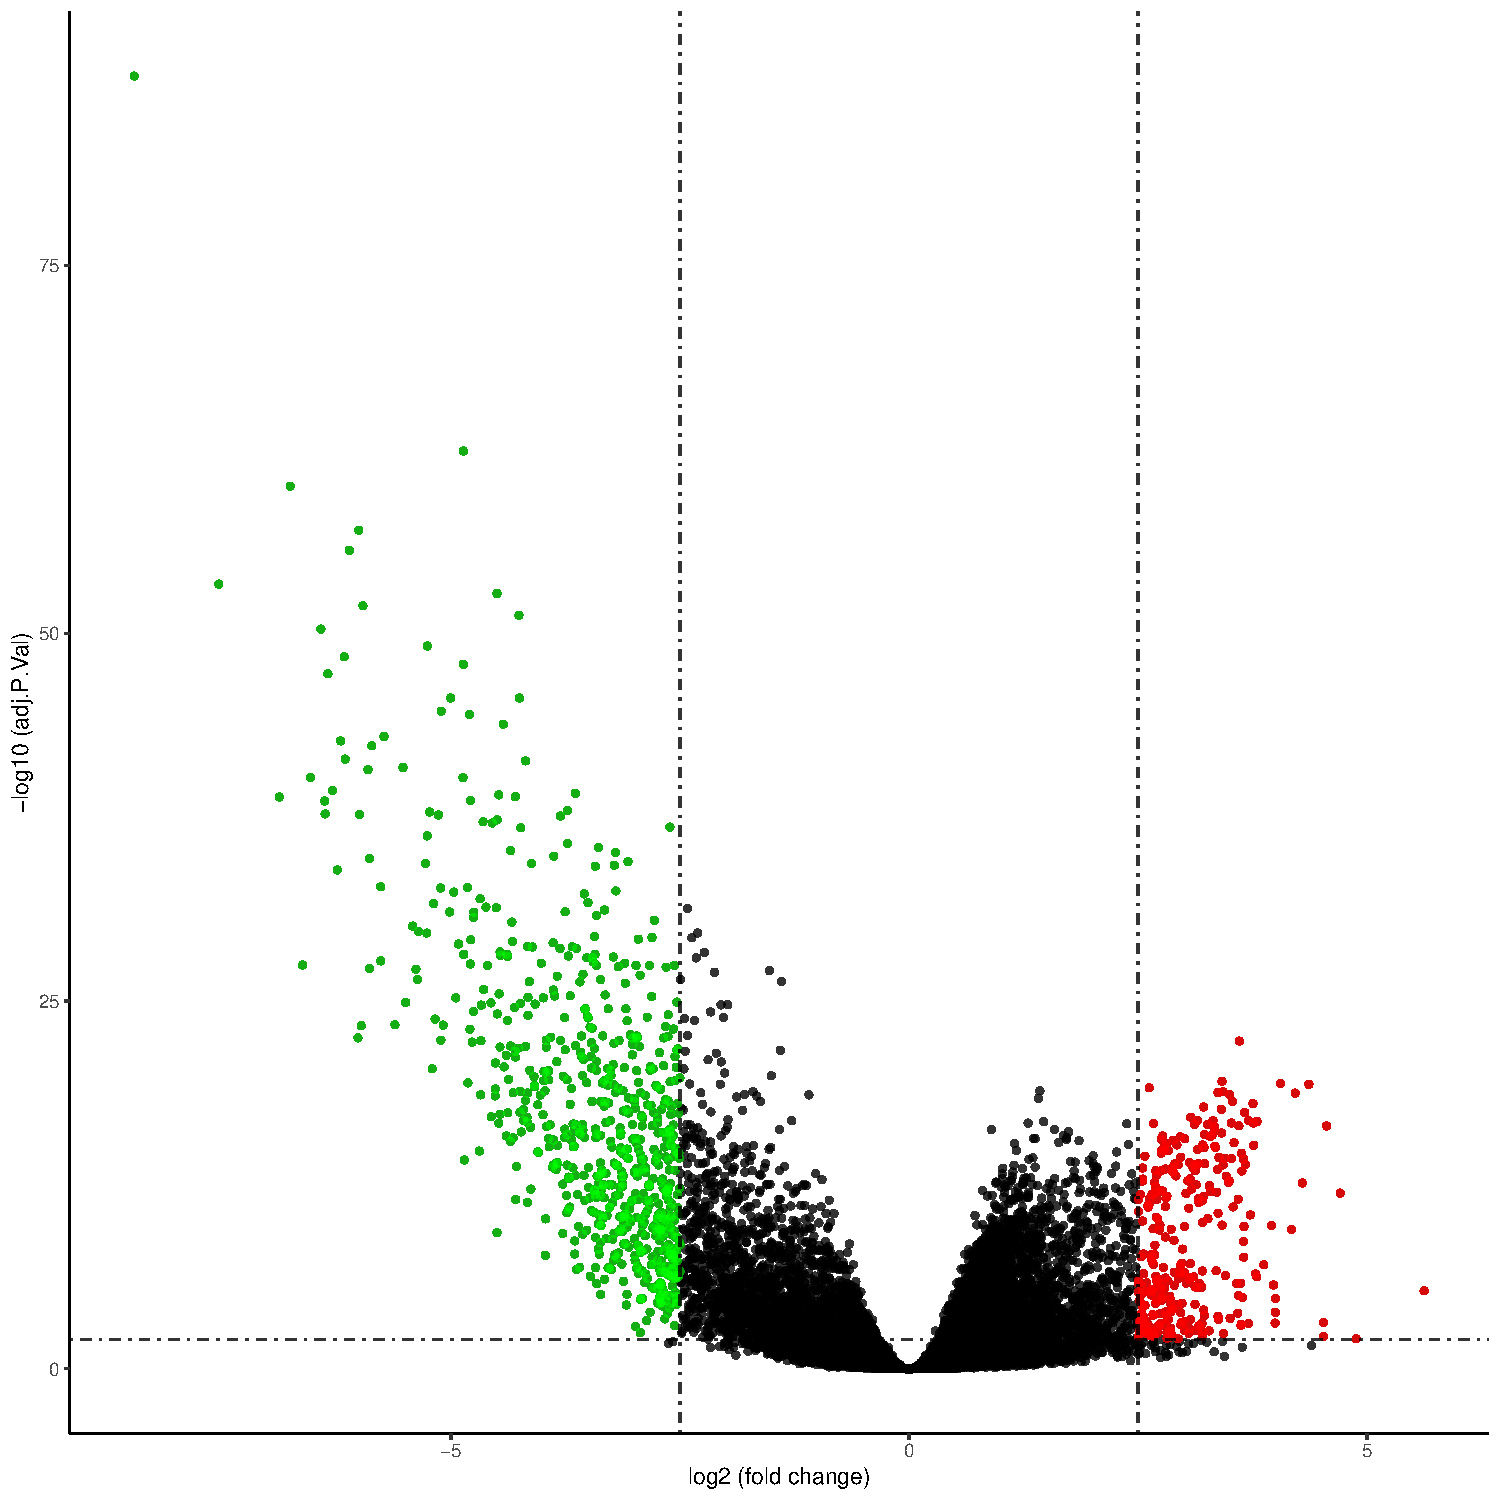
\includegraphics[width=0.6\textwidth]{mRNA_volcano.pdf}
	\caption{mRNA的火山图}
      \label{fig:volcano_mRNA}
\end{figure}
\figref{fig:volcano_mRNA}展示了mRNA的火山图.thesis-NJFU提供\verb|\figref|命令来引用图片.
图片路径为\verb|./pic/|.

\subsection{表格示例}

\begin{table}[htbp]
    \centering
    \caption{部分差异表达基因}
      \begin{tabular}{ccccc}
      \toprule
      GENE\_SYMBOL & logFC & P.Value & adj.P.Val & B \\
      \midrule
      C2orf40 & 9.336405 & 1.87E-13 & 4.32E-09 & 20.23188 \\
      ASB5  & 10.11454 & 3.37E-13 & 4.32E-09 & 19.70257 \\
      RBFOX3 & 10.98724 & 3.79E-13 & 4.32E-09 & 19.59743 \\
      SGCA  & 6.021003 & 1.55E-12 & 1.33E-08 & 18.31813 \\
      SYNPO2 & 7.503317 & 3.34E-12 & 2.28E-08 & 17.6154 \\
      ANGPTL7 & 7.949949 & 4.29E-12 & 2.44E-08 & 17.3859 \\
      PCP4  & 8.485756 & 5.34E-12 & 2.61E-08 & 17.18358 \\
      DACT3 & 5.740747 & 6.99E-12 & 2.99E-08 & 16.93532 \\
      NEXN  & 5.272851 & 8.15E-12 & 3.10E-08 & 16.79358 \\
      \bottomrule
    \end{tabular}%
    \label{tab:degs}%
  \end{table}%
\tabref{tab:degs}展示了部分差异基因.thesis-NJFU提供\verb|\tabref|命令来引用表格.

\subsection{定理示例}
thesis-NJFU提供\verb|lemma|环境来撰写引理.
从上述的例子我们猜想有下述引理\ref{lemma:demo},并且将证明这个猜想是正确的
\begin{lemma}
	设向量组$\beta_1,\beta_2,\cdots,\beta_r$可以由向量组
	$\alpha_1,\alpha_2,\cdots,\alpha_s$线性表出.
	如果$r>s$,那么向量组$\beta_1,\beta_2,\cdots,\beta_r$线性相关.
	\label{lemma:demo}
\end{lemma}
thesis-NJFU提供\verb|proof|环境来撰写证明.
\begin{proof}
	为了证明$\beta_1,\beta_2,\cdots,\beta_r$线性相关,
	就需要找到一组不全为零的数$k_1,k_2,\cdots,k_r$,使得

	...

	因此$\beta_1,\beta_2,\cdots,\beta_r$线性相关.
\end{proof}
thesis-NJFU提供\verb|corollary|环境来撰写推论.
由引理\ref{lemma:demo}立刻得到:
\begin{corollary}
	设向量组$\beta_1,\beta_2,\cdots,\beta_r$可以由向量组
	$\alpha_1,\alpha_2,\cdots,\alpha_s$线性表出.
	如果$\beta_1,\beta_2,\cdots,\beta_r$线性无关,则$r\leqslant s$.
\end{corollary}
thesis-NJFU提供\verb|definition|环境来撰写定义.
\begin{definition}
	向量组的极大线性无关组所含向量的数目称为这个向量组的秩.
\end{definition}
thesis-NJFU提供\verb|proposition|环境来撰写命题.
\begin{proposition}
	向量组$\alpha_1,\alpha_2,\cdots,\alpha_s$线性无关的充分必要条件是
	它的秩等于它所含向量的数目$s$.
\end{proposition}
thesis-NJFU提供\verb|theorem|环境来撰写定理.
\begin{theorem}
	$K^n$的每一个非零子空间$U$都有一个基.
\end{theorem}
thesis-NJFU提供\verb|example|环境来撰写例.
\begin{example}
	设$r<n$.在$K^n$中,令
	\[
	W = \{ (x_1.x_2,\cdots,x_r,0,\cdots,0) | x_i \in K, i=1,2,\cdots,r \}
	\]
	说明$W$是$K^n$的一个子空间,并求$W$的一个基和维数.
\end{example}
thesis-NJFU提供\verb|solution|环境来撰写解.

\begin{solution}
	显然$0\in W$.容易看出$W$对于加法,数量乘法都封闭,因此$W$是$K^n$的一个子空间.
\end{solution}

\section{测试}
\subsection{二级标题}
{\normalsize 字}{\fontsize{12pt}{0pt}\selectfont 字12pt}
{\normalsize 字}{\fontsize{10pt}{0pt}\selectfont 字10pt}
{\normalsize 字}{\fontsize{10.5pt}{0pt}\selectfont 字10.5pt}
{\normalsize 字}{\fontsize{11pt}{0pt}\selectfont 字11pt}

\subsubsection{三级标题}
\begin{equation}
	E = mC^2
\label{eq:relativity}
\end{equation}
质能方程\eqref{eq:relativity}.使用\verb|\eqref|命令来引用公式.
thesis-NJFU采用章节号+公式出现顺序来编号公式.

\begin{equation}
	\mathrm{e}^{i\theta} = \cos \theta + i \sin \theta
\label{eq:Euler}
\end{equation}
Euler公式\eqref{eq:Euler}.

\begin{align*}
	\mathbb{E}\{X_i\} :=& \int\cdots\int x_i \dfrac1{\operatorname{B}(\boldsymbol{\alpha})} \prod\limits_{j=1}^m x_j^{\alpha_j - 1} \, \mathrm{d}x_1 \cdots \mathrm{d}x_m\\
	%=& \int\cdots\int \dfrac1{\operatorname{B}(\boldsymbol{\alpha})} \prod\limits_{\substack{j=1 \\ j\neq i}}^m x_j^{\alpha_j - 1} \cdot x_i^{(\alpha_i+1) - 1} \, \mathrm{d}x_1 \cdots \mathrm{d}x_m\\
	%=& \int\cdots\int \frac{\Gamma\left(\sum\limits_{i=1}^m \alpha_i\right)}{\prod\limits_{i=1}^m \Gamma(\alpha_i)}\prod\limits_{\substack{j=1 \\ j\neq i}}^m x_j^{\alpha_j - 1} \cdot x_i^{(\alpha_i+1) - 1} \, \mathrm{d}x_1 \cdots \mathrm{d}x_m\\
	=& \int\cdots\int \frac{\Gamma\left(\sum\limits_{\substack{j=1 \\ j\neq i}}^m \alpha_j + \alpha_j + 1\right)/{\sum\limits_{j=1}^m \alpha_j}}{\prod\limits_{\substack{j=1 \\ j\neq i}}^m \Gamma(\alpha_j) \cdot \Gamma(\alpha_i + 1) / \alpha_i}\prod\limits_{\substack{j=1 \\ j\neq i}}^m x_j^{\alpha_j - 1} \cdot x_i^{(\alpha_i+1) - 1} \, \mathrm{d}x_1 \cdots \mathrm{d}x_m\\
	=& \dfrac{\alpha_i}{\sum\limits_{j=1}^m \alpha_j} \int\cdots\int \frac{\Gamma\left(\sum\limits_{\substack{j=1 \\ j\neq i}}^m \alpha_j + \alpha_j + 1\right)}{\prod\limits_{\substack{j=1 \\ j\neq i}}^m \Gamma(\alpha_j) \cdot \Gamma(\alpha_i + 1)}\prod\limits_{\substack{j=1 \\ j\neq i}}^m x_j^{\alpha_j - 1} \cdot x_i^{(\alpha_i+1) - 1} \, \mathrm{d}x_1 \cdots \mathrm{d}x_m
\end{align*}
注意到上式中被积函数为$\operatorname{Dirichlet}(\alpha_1,\cdots,\alpha_i+1,\cdots,\alpha_m)$的密度函数,其积分结果为1,因此
\[
	\mathbb{E}\{X_i\} = \dfrac{\alpha_i}{\sum\limits_{j=1}^m \alpha_j}
\]

仓库的运作是物流的第一步,仓库的运作效率直接影响整个物流活动的效率,
而拣货作业是仓库的核心作业之一,电商订单又有个性化程度高、批量小、频率高等特点,
因此优化拣货路径是有必要的。本文就某公司仓内拣货路径问题进行分析,给出其最优方案。

针对问题一,我们将距离问题分为三类:货格间的距离,复核台与货格间的距离
以及复核台与复核台之间的距离。其中我们将货格间的距离又细分为跨行距离,
跨巷道距离和不跨行不跨巷道距离。并且我们将仓库进行抽象并定义了一些特征,
然后给出了货架号,货格号数字部分与特征之间的计算公式。最后使用MATLAB
程序实现了输入元素编号并得出其间的距离。


针对问题二,由于任务单中的货物较多,我们使用了蚁群算法来减少运算量,
并取得了较好的效果。在第一问所得的相关公式与程序的帮助下很快地得到了距离矩阵。
由于结束的复核台不确定,我们分别求出了在各个复核台结束的最短路径并进行了比较,
最后得出最优路径,路线的示意图已在下文给出。最优路径长度为381600mm,
返回的复核台为FH07,完成出库总共花费时间为461.4s。

针对问题三,我们首先将完成任务单的过程抽象成有向图。我们可以通过蚁群算法
得出每条边的长度,由此我们可以使用动态规划模型求出其最小值。对于任务单的顺序,
我们对其进行了枚举,得出最优规划为依次领取任务T0006,T0005,T0003,T0004,T0002,
完成出库总计需要花费时间2400s,复核台FH03,FH11的利用率分别为6.1576\%,6.3939\%。

针对问题四,由于本题解空间过于复杂,精确求出最优解是不必要的,
我们巧妙地以较小代价求出一个尽可能好的解。不妨为每个拣货员随机分配一个初始复核台,
并计算出完成任务单的最短路径,然后为其分配最近的复核台。最终通过MATLAB程序计算出完成
楚克需要花费的时间为2991.8s。

\conclusion
结论内容

\acknowledgement
致谢内容

\thesisreferences

\end{document}